\chapter{Volume Average Method}
\label{ch:vans}

\chapquote{Do not worry about your difficulties in mathematics; I can assure you that mine are still greater.}{Letter to junior high school student Barbara Wilson, \\ January 7, 1943}{Albert Einstein}

\section{Introduction}

In the previous chapter we have already introduced the volume averaging method and how it can be used to derive a macroscopic description of the microscopic system of equations.
The homogenized version of the system is valid everywhere in the porous medium domain, and not only in the fluid phase.
Theoretical aspect of the volume averaging method can be found in \citet{whitaker2013method}, \citet{whitaker1986flow}, \citet{whitaker1996forchheimer}, \citet{quintard1994transport1}, \citet{quintard1994transport2}, \citet{quintard1994transport3}, \citet{quintard1994transport4}, \citet{quintard1994transport5} and many others contributions that are introduced in the next chapter.
The various steps necessary to derive the local average version of the fluid dynamic equations are listed in the following.

\section{Homogenization procedure}
The mathematical method of volume averaging is based on some fundamental steps that one should follow in order to retrieve the homogenized version of the equations.
The main steps are:
\begin{itemize}
\item Definition of the averaging operator
\item Use of theorems that permits to interchange the derivation and the averaging operation
\item Decomposition of fields as a sum of mean field and a perturbed field
\item Assumption of length-scales constraints (based on the problem definition) that help to simplify and define a local closure  problem
\end{itemize}

Such schema is graphically resumed in \citet{paez2017macroscopic} and \citet{davit2013homogenization}. A similar flowchart of the complete overall procedure is showed in figure \ref{fig:schema_vans_homo}.

\begin{figure}[h!]
	\centering
	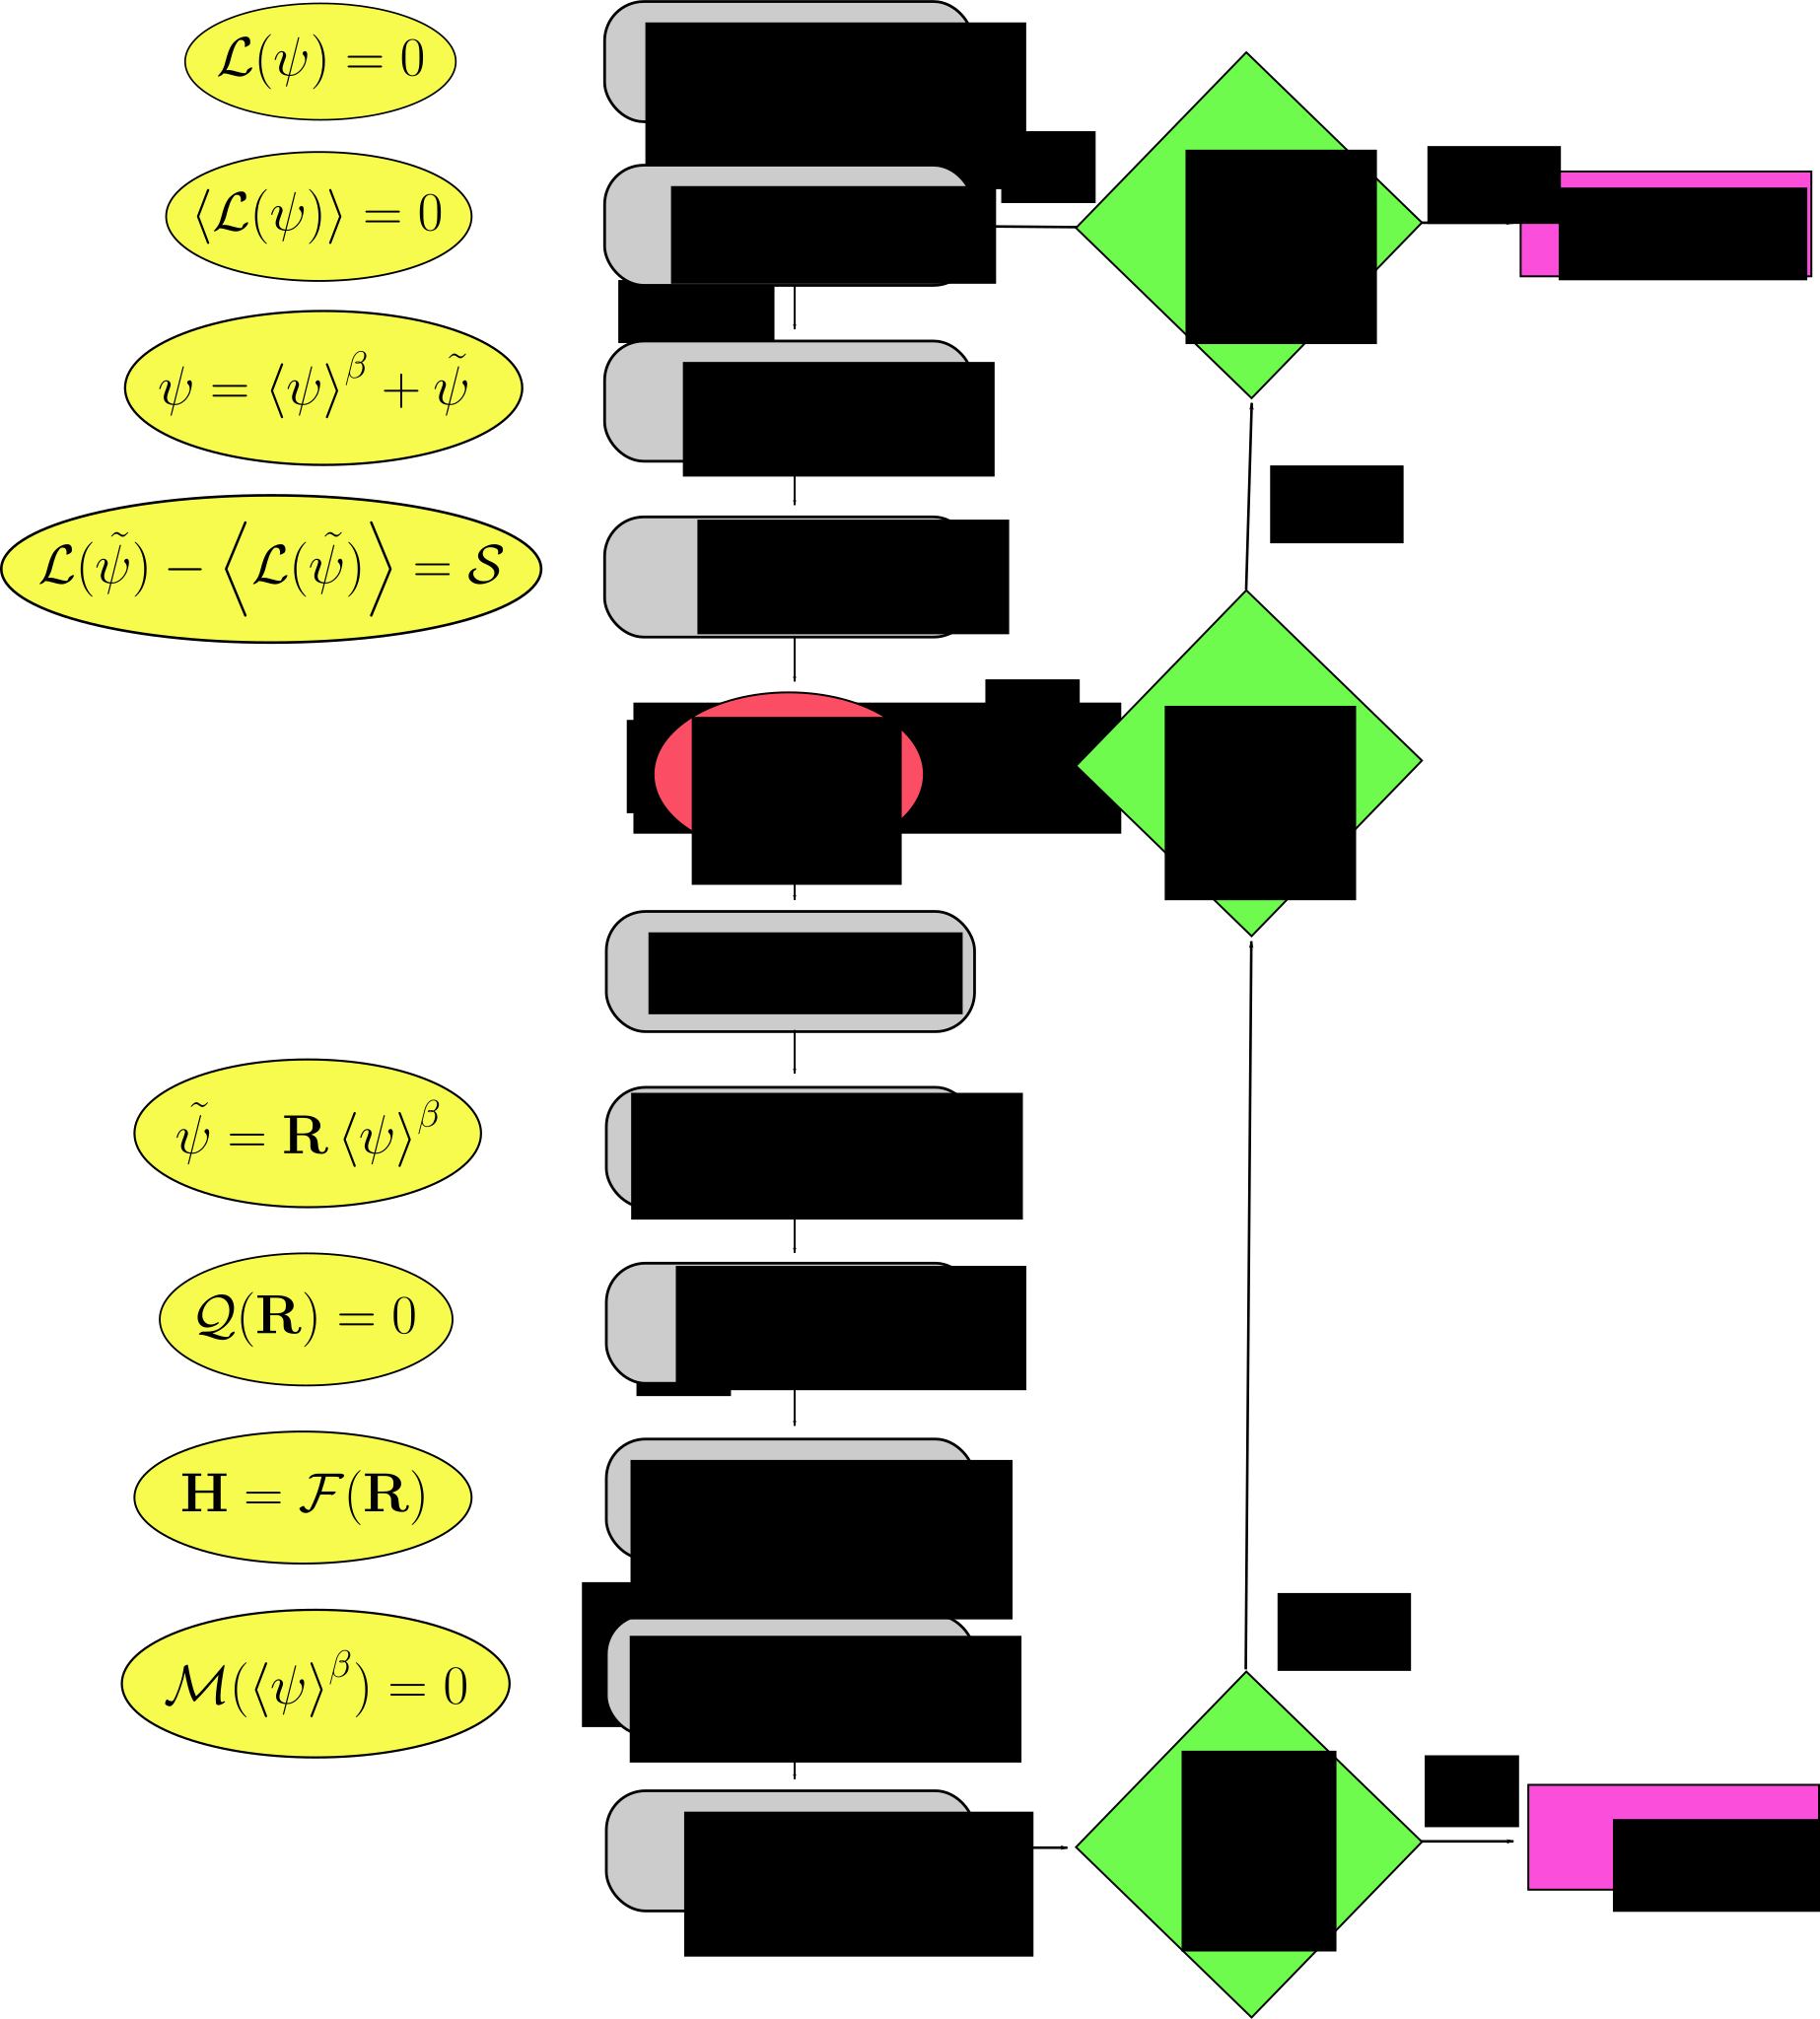
\includegraphics[width=0.95\textwidth,height=0.95\textheight,keepaspectratio]{chapter_2/figure/schema}
	\caption{Illustration of the volume average homogenization procedure. Image adapted from \citet{davit2013homogenization}}
	\label{fig:schema_vans_homo}
\end{figure}

\section{Derivation of VANS equations for 3D incompressible fluids}
\subsection{Navier-Stokes equations}
The dynamic of the fluid phase (indicated with the subscript $\beta$), inside and above the porous medium, is governed by the Navier-Stokes equation for incompressible Newtonian fluid:

\begin{eqnarray}
	\begin{cases}
		\dfrac{\partial \vb}{\partial t} +  \nabla \cdot (\vb \vb)  = -\dfrac{1}{\rho_{\beta}} \nabla \pb + \nub \nabla^2  \vb  \\
		\nabla \cdot \vb = 0 \\
		\vb = \ws \quad \text{at} \; A_{\beta\sigma}
	\end{cases}
\label{eq:NS}
\end{eqnarray}\\

where $\vb$, $\pb$, $\rho_{\beta}$ and $\nub$ stand, respectively, for  the velocity, the pressure, the density and the kinematic viscosity of the fluid.
The interface between the fluid and the solid is indicated as $A_{\beta\sigma}$, in which the no-slip condition for the velocity apply.
In the above boundary condition $\ws$ is the velocity of the solid phase.
Initial condition should also be specified in order to solve the system, but they do not take active part in the homogenization procedure.
The next sections shows how to average this system using the volume average method.

\subsection{Definition of the averaging operators}
Figure \ref{fig:rev} show the schematics of the internal structure of a fibrous porous medium, the important quantities are also indicated in the same picture.
The shape of the volumes used in the averaging operations are enclosed in continuous lines. $V|_{\mathbf{x}}$ indicate the volume with centroid $\mathbf{x}$ and $V_{\beta}|_{\mathbf{x}}$ indicate the fluid volume fraction inside the latter.
The coordinate $\mathbf{r} = \mathbf{x} +\mathbf{y}$ represent the centroid of another possible volume in which one can compute the average quantities, the boundaries of the same volume are indicated with dotted lines.

\begin{figure}[h!]
	\centering
	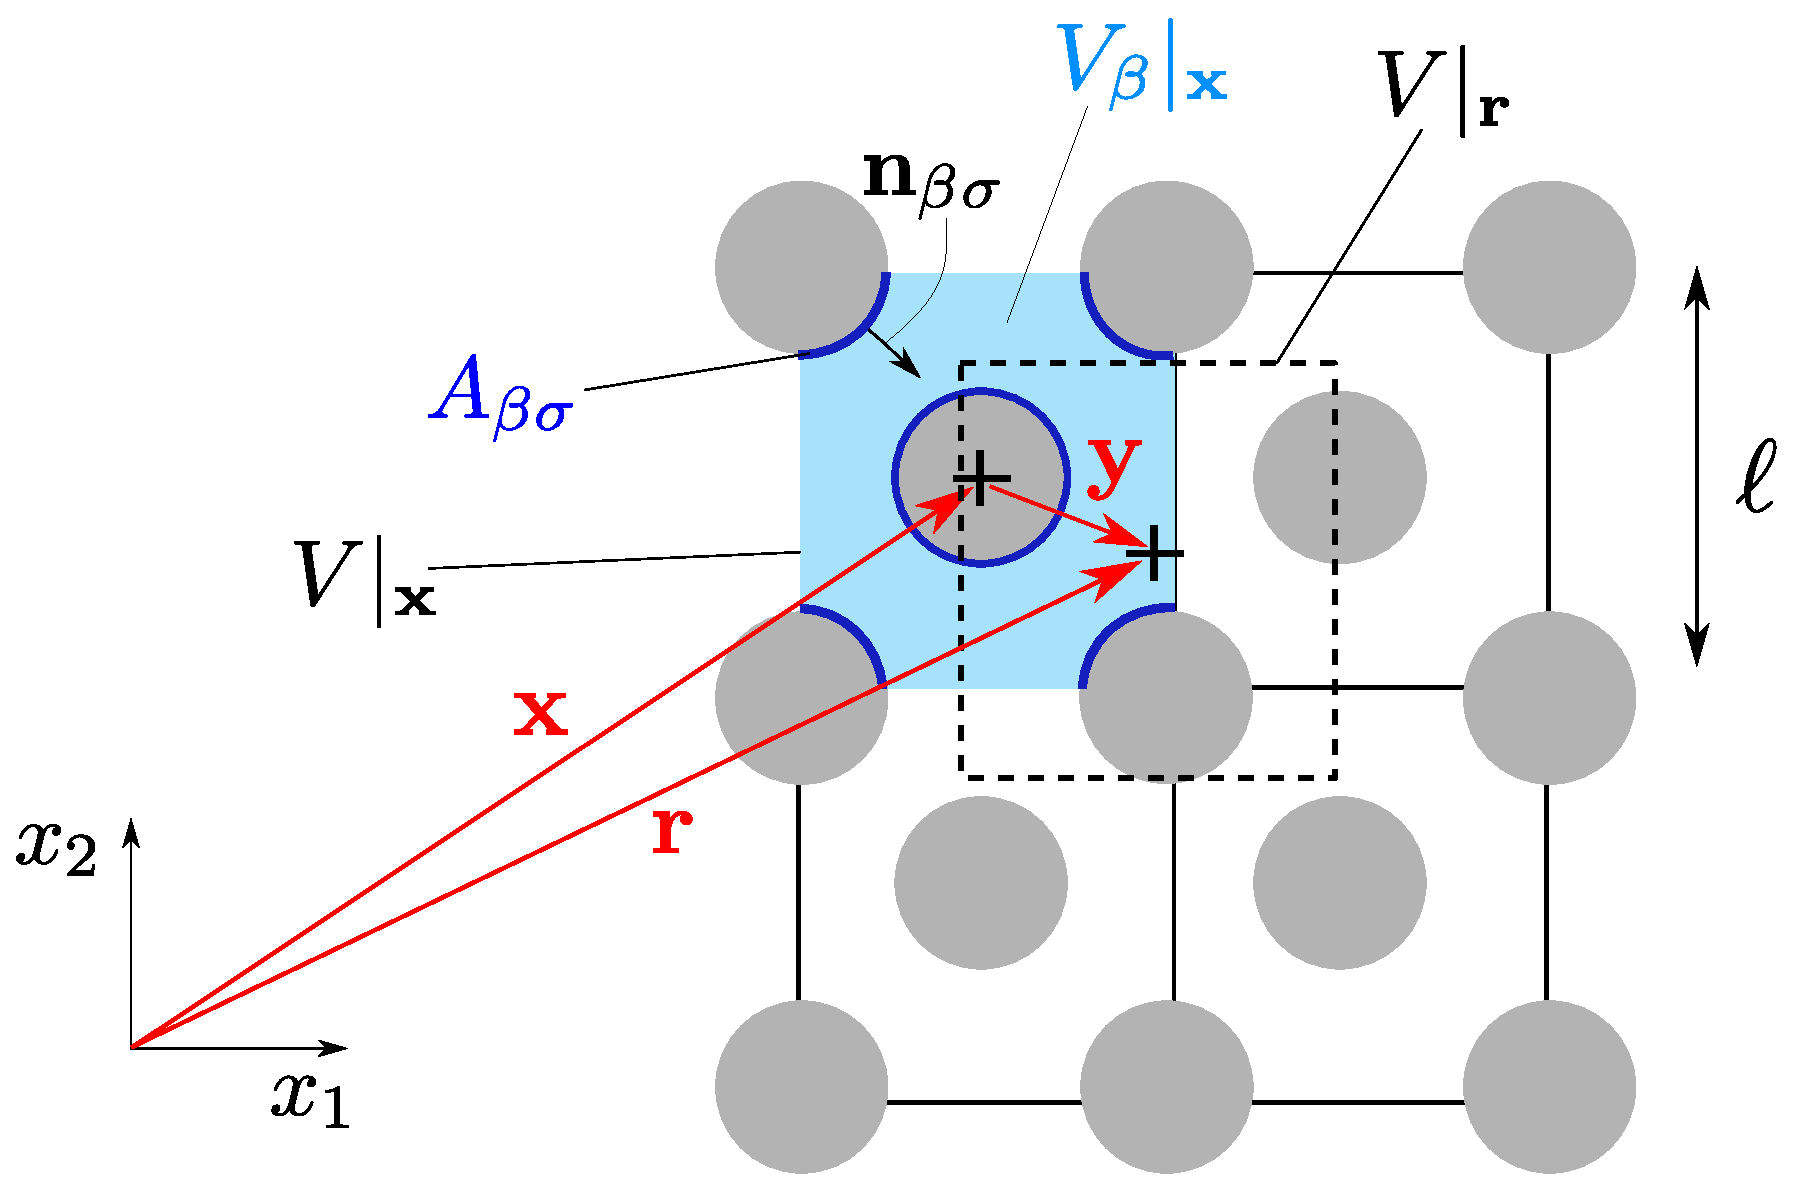
\includegraphics[width=0.7\linewidth]{chapter_2/figure/REV}
	\caption{A graphic representation of the averaging volumes and interfaces in case of fibrous (ordered) porous media. In this example the fibers are in staggered arrangement. The edges of the volumes that have centroid position $\mathbf{x}$ are shown in continuous lines and the ones with centroid $\mathbf{r}$ are shown in dotted lines.}
	\label{fig:rev}
\end{figure}

Let $\psi_{\beta}$ be a an arbitrary order tensors (scalar, vector or second order tensor) defined in the fluid phase of the volume $V$ with $\mathbf{x}$ as centroid.

\newpage 

$\quad$

\newpage

Two different volume averaging operators should be defined, the \textit{intrinsic average} indicated as $\meani{.}$ reads:

\begin{equation}
	\meani{\psi_{\beta}}|_{\mathbf{x}} = \dfrac{1}{\volb(\mathbf{x})} \int_{\volb(\mathbf{x})}  m(\mathbf{y}) \psi_{\beta}(\mathbf{x}+\mathbf{y}, t) d \, \volb,
	\label{eq:avg_intrinsic}
\end{equation}

where $m$ is a weight function defined on $\volb$ and $\mathbf{y}$ is the relative position vector with respect to the centroid $\mathbf{x}$ of the averaging volume $\volb$.

The second one is the \textit{superficial average} indicated with $\means{}$:
\begin{equation}
	\means{\psi_{\beta}}|_{\mathbf{x}} = \dfrac{1}{V} \int_{\volb(\mathbf{x})} m(\mathbf{y}) \psi_{\beta}(\mathbf{x}+\mathbf{y}, t) d \, \volb,
	\label{eq:avg_superficial}
\end{equation}

In the two definition $\mathbf{y}$ is the integration variable.
The difference between the two formulations is that the former takes into account the actual fluid fraction in averaging the filed instead of the pure size of the total volume.

In order to use a less heavy notation, the subscript $|_{\mathbf{x}}$ is dropped in the following procedure, but should be kept in mind that the volume averaged quantities are explicitly dependents on the center position of the volume as both averaging operators are defined as a volume integral.
The size and shape of the integration domain can also be problematic and more details on this issues are presented in the paragraphs \ref{ch:filter}.

In the definition of the average operators is possible to introduce a weight function ($m$), that has the aim to guarantee smooth volume averaged fields.
However, the choice of his formulation depends on the porous media geometry, as the size of the average volume.

The notation is further simplified if a constant weight is considered ($m=1/V$), in such case it is possible to drop it from the average operators.
However any shape of the function $m$ can be used without formally change the final form of the averaged equation.

The porosity of a porous medium cell is defined as:
\begin{equation}
	\varepsilon = \dfrac{\volb}{V}
	\label{eq:porosity}
\end{equation}
which represent how much fluid is actually present inside the averaging volume, in other terms it is an indication of how packed are the fibers of our porous media.

Using the above definition, it is possible to express a relationship between the two averaging operators:
\begin{equation}
	\means{\psi_{\beta}} =  \varepsilon \meani{\psi_{\beta}}
	\label{eq:means_vs_meani}
\end{equation}

\subsection{Choice of shape and size of averaging volume and weight function}
\label{ch:filter}

The problem of choosing the right weight function, for a give geometry of the porous medium, has been extensively studied by the series of works \citet{quintard1994transport1}, \citet{quintard1994transport2}, \citet{quintard1994transport3}, \citet{quintard1994transport4}, \citet{quintard1994transport5} and more recently generalized by \citet{davit2017technical}.

The authors above differentiate their results for ordered and disordered porous medium. They show that in each case a specific size and shape of the weight function (and the volume) is needed.
The volume in which the average procedure is applied is called \textit{reference elementary volume} (REV).
Usually for disordered porous media a spherical volume is the most appropriate, and the REV size ($\ell$) should satisfy the length scale constraint:
$$
\ell_{\beta} \ll \ell \ll L
$$
where $\ell_{\beta}$ is a characteristic distance of the pore spacing.
Instead in case of ordered porous media the most appropriate shape is usually a cube with side:
$$
O(\ell_{\beta}) = \ell \ll L
$$
The above constraint can be reinterpreted as the separation of scale parameter in the multiple scale method $\epsilon = \ell/L \ll 1$.

\citet{ochoa1995momentum} confirm the same length-scale constraints even in case of an interface between a free fluid and a porous medium.

The size of the REV ($\ell$) should be chosen with the above specifications. These length scale constraints ensure that the volume is large enough that periodic boundary condition can be applied in the exterior of the volume. Anyhow the REV size should also capture all the phenomena that take place at the micro-scale ($\ell_{\beta}$).
If the REV size is the correct one, increasing or decreasing its size should not change the averages quantities. The weight function can also help to attenuate variation of the averaged fields due to geometrical inhomogenities of the porous medium. As a matter of fact, it acts as a low-pass filter for the perturbations fields.

The weight function can  also play an important role in the interpretation of the averaged equation. As showed later on, in order to retrieve a local form of the VANS equations, the following statement should in principle has to be true:
\begin{equation}
\Big\langle \means{\psi_{\beta}}|_{\mathbf{r}}  \Big\rangle  |_{\mathbf{x}} = \means{\psi_{\beta}}|_{\mathbf{x}}
\label{eq:well_behaved}
\end{equation}
It means that the averaged field contain small variations at the micro-scale (inside the averaging volume $V$).
In order to satisfy this requirement certain weight function can perform better than others, although the same conclusion can be derived from the length-scales constraints.
In paragraph \ref{ch:appendix_a}, at the end of this chapter, some details of this approximation are further explained.

For disordered porous medium the \textit{hat function} $m^{\sqcap}$ which has the form:
\begin{eqnarray}
	m^{\sqcap}(\mathbf{y}) 
	\begin{cases}
		\dfrac{1}{V} \quad &|\mathbf{y}| \leqslant r_0\\
		0 \quad &|\mathbf{y}|> r_0
	\end{cases}
\end{eqnarray}
can be used to produce smooth averaged fields.

Instead for ordered porous medium the literature shows that triangle shaped functions called \textit{cellular filter}  $m^{\bigtriangleup}$  performs better:
\begin{eqnarray}
m^{\bigtriangleup}(\mathbf{y}) 
\begin{cases}
(\ell/2 - |\mathbf{y}|) \quad &|\mathbf{y}| \leqslant r_0\\
0 \quad &|\mathbf{y}|> r_0
\end{cases}
\end{eqnarray}

\citet{davit2017technical} had recently expanded the required hypothesis that a $m$ function should satisfy. In general the weight function $m$ should:
\begin{itemize}
	\item be normalized in as: $\displaystyle\int_{\volb}  m(\mathbf{y}) \; d\volb = 1$
	\item have compact support 
	\item satisfy: $m*\psi_{\beta} \in C^{k}$, where $k$ represent the order of the closure
	\item satisfy: $(m \, \mathcal{P}^j(\mathbf{y}))*\psi_{\beta}
	\begin{cases}
	0 \quad &\textrm{if}\quad \textrm{j} \; \textrm{odd}\\
	const  \quad &\textrm{if}\quad \textrm{j} \; \textrm{even}
	\end{cases}$
\end{itemize}

Where $\mathcal{P}^j(\mathbf{y})$ is a polynomial of order $j$.
The last requirement uses the fact that the average operation can also be defined as a convolution product between the weight function and the flow field quantities (\citet{marle1982macroscopic}):
$$
\means{\psi_{\beta}}|_{\mathbf{x}} = \dfrac{1}{V} \int_{\volb(\mathbf{x})} m(\mathbf{y}) \psi_{\beta}(\mathbf{x}+\mathbf{y}, t) d \, \volb = m*\psi_{\beta}
$$

The choice of the weight function shape is very important, however previous works in which the authors had implicitly used $m^{\sqcap}$ are not wrong.
As a matter of fact, if the assumption of well behaved fields hold \footnote{it means that the equation \eqref{eq:well_behaved} can be verified a posteriori} then the homogenized equations are the correct one.
However neglecting the use of the proper weight function can induce some problem on the interpretations of the averaged fields \footnote{as \citet{quintard1994transport1} show for the example case of hydrostatic pressure}, as a consequence particular care should be used especially when making comparison to experiments.

In the following derivation of the equation no weight function is used inside the averaged operators, in order to not make the notation heavier.
In any case in the following text is indicated whenever this special hypothesis on the weight function is needed.

\subsection{Theorems involving derivatives of spatial averaged quantities}

The purpose of these theorems is to be able to swap the derivative and the volume average operation.

\begin{theorem}[Spatial averaging theorem]
Let $\psi_{\beta}$ be a scalar quantity defined in the fluid phase $\beta$, then:

	\begin{equation}
		\means{\nabla \psi_{\beta}} = \nabla \means{\psi_{\beta}} + \dfrac{1}{V} \int_{A_{\beta \sigma}} \psi_{\beta} \nbs   \;dA
			\label{th:spat_avg}
	\end{equation}
\end{theorem}

In the above $\means{\psi_{\beta}}$ is evaluated at $\mathbf{x}$ and the operator $\nabla$ express the differentiation operation in respect to $\mathbf{x}$ also.

\begin{corollary}[Vector form of \eqref{th:spat_avg}]
	The vector form of the spatial averaging theorem is given by:
	
	\begin{equation}
	\means{\nabla \cdot \boldsymbol{\psi}_{\beta}} = \nabla \cdot \means{ \boldsymbol{\psi}_{\beta}} + \dfrac{1}{V} \int_{A_{\beta \sigma}}  \boldsymbol{\psi}_{\beta} \cdot \nbs \;dA
			\label{th:vec_spat_avg}
	\end{equation}
\end{corollary}

\begin{corollary}
	Applying the theorem \eqref{th:spat_avg} to a constant field $\psi_{\beta} = 1$ the following relation can be found:
	
	\begin{equation}
		\nabla \varepsilon = - \int_{A_{\sigma \beta}} \nbs d \, A,
	\end{equation}
\end{corollary}

\newpage

\begin{theorem}[Reynolds transport theorem]
	Let $\psi_{\beta}$ be a quantity defined in the fluid phase $\beta$, then:
	
	\begin{equation}
	\dfrac{\partial}{\partial t} \int_{\volb(t)} \psi_{\beta} \; dV =  \int_{\volb(t)} \dfrac{\partial \psi_{\beta}}{\partial t} \; dV + \int_{A_{\beta \sigma}(t)} \psi_{\beta} ( \mathbf{\ v}_{\sigma} \cdot \mathbf{n}_{\beta \sigma} ) \;dA,
	\label{th:transport}
	\end{equation}
	
	where $\mathbf{\ v}_{\sigma}$ is the point velocity of the solid-fluid interface $A_{\beta \sigma}$.
\end{theorem}

The three theorems and the corollary are essential to develop the closed form of the equations.
One interesting thing to pay attention is that the theorems switch the average and derivative operation but always introduces a non local integral term.

\subsection{Averaged continuity equations}
We start by finding the averaged version of the continuity equation in \eqref{eq:NS}:

\begin{equation}
\means{\nabla \cdot \vb}   = 0
\label{eq:superf_avg_cont}
\end{equation}

Applying theorem \eqref{th:spat_avg} to the previous equation we get:
$$
\means{\nabla \cdot \vb} = \nabla \cdot \means{\vb} + \dfrac{1}{V} \int_{A_{\beta \sigma}}  \vb \cdot \nbs \;dA
$$
The boundary condition at the interface ($\ws = \vb$) implies that the integral above can be modified: 
$$=\nabla \cdot \means{\vb} + \dfrac{1}{V} \int_{A_{\beta \sigma}}  \ws \cdot \nbs \;dA$$
Now we rewrite the last term as if it was a result of the Reynolds transport theorem applied to a constant unitary scalar field:
$$=\nabla \cdot \means{\vb} + \derp{}{t} \dfrac{1}{V} \int_{\volb} \;dV  - \dfrac{1}{V} \int_{\volb} \derp{1}{t} \;dV $$
where the last integral is zero due to the time derivation of a constant field. The first term can be further developed, obtaining finally the averaged continuity equation:

\begin{equation}
\nabla \cdot \means{\vb} + \derp{\varepsilon}{t} =0
\label{eq:avg_1}
\end{equation}


\subsection{Averaged momentum equations}
We seek the average version of the momentum equation in \eqref{eq:NS} re-showed below:

\begin{equation}
\dfrac{\partial \vb}{\partial t} + \nabla \cdot (\vb\vb) = -\frac{1}{\rho_{\beta}} \nabla \pb + \nub \nabla^2  \vb
\label{eq:mom_1}
\end{equation}

In order to keep the procedure readable the development of each term is performed separately, in the same order as they appear in equation \eqref{eq:mom_1}.

\subsubsection{Temporal derivative term}
Using theorem \eqref{th:transport} we can rewrite the first term of the equation as:

\begin{equation}
\means{\derp{\vb}{t}} = \derp{\means{\vb}}{t} -\dfrac{1}{V} \int_{A_{\beta \sigma}}  \vb (\ws \cdot \nbs )\;dA
\end{equation}

\subsubsection{Convective term}
Theorem \eqref{th:vec_spat_avg} applied to the convective term gives us:

\begin{equation}
\means{\nabla \cdot (\vb\vb)} = \nabla \cdot \means{\vb \vb} + \dfrac{1}{V} \int_{A_{\beta \sigma}}  (\vb \vb) \cdot \nbs \;dA
\end{equation}

The boundary condition at the interface ($\ws = \vb$) implies that the integrals inside the convective and temporal part are equal, so the total left end side of the momentum equation became:

\begin{equation}
\text{LHS} = \derp{\means{\vb}}{t} + \nabla \cdot \means{\vb \vb}
\label{eq:lhs}
\end{equation}

\subsubsection{Pressure term}
The pressure term is also expanded using theorem \ref{th:spat_avg}:

\begin{equation}
\means{-\dfrac{1}{\rho_{\beta}} \nabla \pb } = -\dfrac{1}{\rho_{\beta}} \nabla \means{\pb} -\dfrac{1}{V} \int_{A_{\beta \sigma}}  \dfrac{\pb}{\rho_{\beta}}  \cdot \nbs \;dA
\end{equation}

\subsubsection{Diffusion term}
Here we fist use the identity $\nabla^2 = \nabla \cdot (\nabla)$ \footnote{laplacian = div(grad)}, then we apply the theorem \ref{th:vec_spat_avg} directly to this expansion to get:

\begin{equation}
\means{\nub\nabla^2 \vb} = \means{\nub\nabla \cdot \nabla \vb} = \nabla \cdot \means{\nub\nabla \vb} +\dfrac{1}{V} \int_{A_{\beta \sigma}}  \nub \nabla \vb \cdot \nbs \;dA
\label{eq:4_1}
\end{equation}

Now using the theorem \ref{th:vec_spat_avg} on $\means{\nabla \vb}$ we get:

\begin{eqnarray}
	\means{\nub\nabla^2 \vb} &=& \nabla \cdot \nub \nabla \means{\vb} + \nabla \cdot \left( \dfrac{1}{V} \int_{A_{\beta \sigma}}  (\nub \vb) \cdot \nbs \;dA \right) + \dfrac{1}{V} \int_{A_{\beta \sigma}} \left( \nub \nabla \vb \right) \cdot \nbs \;dA  \nonumber \\
	&=& \nub\nabla^2 \means{\vb} +  \nabla \cdot \left( \dfrac{1}{V} \int_{A_{\beta \sigma}}  (\nub \vb) \cdot \nbs \;dA \right) + \dfrac{1}{V} \int_{A_{\beta \sigma}} \left( \nub \nabla \vb \right) \cdot \nbs \;dA,   \nonumber
\end{eqnarray}
using Gauss theorem on the second term we get:
\begin{equation*}
	\means{\nub\nabla^2 \vb} = \nub\nabla^2 \means{\vb} +  \nabla \cdot \left( \dfrac{1}{V} \int_{\volb} \nabla \cdot \left( \nub \vb \right) dV \right) + \dfrac{1}{V} \int_{A_{\beta \sigma}} \left( \nub \nabla \vb \right) \cdot \nbs \;dA,  
\end{equation*}
the second term is zero due to the continuity equation, so the viscous term yields:
\begin{equation}
	\means{\nub\nabla^2 \vb} = \nub\nabla^2 \means{\vb} + \dfrac{1}{V} \int_{A_{\beta \sigma}} \left( \nub \nabla \vb \right) \cdot \nbs \;dA
\end{equation}

%\Red{The above use of the Gauss theorem, to prove that the first integral term is zero, can be bypassed in case of rigid porous media. Which due to the b.c. at the fluid-solid is zero.}

Before continuing the development, by summing all the terms together we get:

\begin{eqnarray}
&& \derp{\means{\vb}}{t} + \nabla \cdot \means{\vb \vb} = -\dfrac{1}{\rho_{\beta}} \nabla \means{\pb} + \nub\nabla^2 \means{\vb} + \nonumber \\
&& +\dfrac{1}{V} \int_{A_{\beta \sigma}} \left( -\dfrac{\pb}{\rho_{\beta}} \mathbf{I} + \nub \nabla \vb  \right)\cdot \nbs \;dA \nonumber \\
\label{eq:mom_2}
\end{eqnarray}

This is still not the averaged version of the momentum equation, since it has the presence of the non-homogeneous term $\means{\vb\vb}$ and the integral term still has the local (microscopic) variables inside.
In the next section these two terms are treated in order to make them function of the only averaged quantities.

\subsection{Length scale decomposition}

The decomposition proposed by \citet{gray1975derivation} is now used to get the average version of the problem \eqref{eq:NS}:

\begin{equation}
\psi_{\beta}(\mathbf{r},t) = \meani{\psi_{\beta}}|_{(\mathbf{r},t)} + \tilde{\psi}_{\beta}(\mathbf{r},t),
\label{eq:gray}
\end{equation}

where $\tilde{\psi}_{\beta}$ is the microscopic scale contribution and $ \meani{\psi_{\beta}}$ the volume average one.  The two contributions should be added together to obtain the local filed value for the considered quantity $\psi_{\beta}$.
This decomposition has been introduced in order to separate the different scales of the spatial variation of the fields, and so separate the low frequencies from the high one.

If the hypothesis of that this division holds, it is possible to demonstrate that the average value of the perturbation field is null \footnote{the paragraph \ref{ch:appendix_a} specifically addresses the hypothesis behind this result}:
$$
\means{\tilde{\psi}_{\beta}} = \means{\psi_{\beta}} - \means{\meani{\psi_{\beta}}} \approx \means{\psi_{\beta}} -\varepsilon \meani{\psi_{\beta}} = \means{\psi_{\beta}} -\means{\psi_{\beta}} = 0
$$


Using the above results, the non-homogeneous term in equation \eqref{eq:mom_2} can be converted in:

\begin{equation}
\means{\vb\vb} = \means{\means{\vb}\meani{\vb}} +2\means{\meani{\vb}\vbt} +\means{\vbt \vbt} = \varepsilon \meani{\vb}\meani{\vb} +\means{\vbt\vbt}
\label{eq:dec_1}
\end{equation}

For each integral term of \eqref{eq:mom_2} the same field decomposition should be applied:

\begin{eqnarray}
\dfrac{1}{V} \int_{A_{\beta \sigma}}  - \left( \dfrac{\pb}{\rho_{\beta}} \mathbf{I} \right) \cdot \nbs \;dA &=& \dfrac{1}{V} \int_{A_{\beta \sigma}}  -\dfrac{1}{\rho_{\beta}} \left(\meani{\pb}   + \pbt \right)  \nbs \;dA  \nonumber \\
&=& +\dfrac{1}{\rho_{\beta}}\nabla\varepsilon \; \meani{\pb} - \dfrac{1}{V} \int_{A_{\beta \sigma}}  \dfrac{\pbt}{\rho_{\beta}}  \nbs \;dA
\end{eqnarray}


\begin{eqnarray}
\dfrac{1}{V} \int_{A_{\beta \sigma}} \nub \nabla \vb \cdot \nbs \;dA &=& \dfrac{1}{V} \int_{A_{\beta \sigma}} \nub \nabla (\meani{\vb} +\vbt) \cdot \nbs \;dA   \nonumber \\
&=& - \nub \nabla \varepsilon \; \nabla \meani{\vb} + \dfrac{1}{V} \int_{A_{\beta \sigma}} \nub \nabla \vbt \cdot \nbs \;dA
\end{eqnarray}

%\begin{eqnarray}
%&&\nabla \cdot \left( \dfrac{1}{V} \int_{A_{\beta \sigma}} \nbs \cdot \nub \vb \;dA \right) = \nabla \cdot \left( \dfrac{1}{V} \int_{A_{\beta \sigma}} \nbs \cdot \nub (\meani{\vb} +\vbt) \;dA \right) =  \nonumber \\
%&=& -\nabla \cdot \left( \nub \meani{\vb} \nabla \varepsilon \right) + \dfrac{1}{V} \nabla \cdot \left(\int_{A_{\beta \sigma}}  \nub \nbs \vbt \;dA \right) =  \nonumber \\
%&=& -\nub  \nabla  \meani{\vb} \nabla \varepsilon -\nub \meani{\vb} \nabla^2 \varepsilon + \dfrac{1}{V} \nabla \cdot \left(\int_{A_{\beta \sigma}}  \nub \nbs \vbt \;dA \right)
%\end{eqnarray}

The momentum equation now reads:

\begin{eqnarray}
\derp{\means{\vb}}{t} + \nabla \cdot (\varepsilon \meani{\vb}\meani{\vb}) + \nabla \cdot (\means{\vbt\vbt}) = -\dfrac{1}{\rho_{\beta}} \nabla \means{\pb} + \nub\nabla^2 \means{\vb} + \nonumber \\
\qquad \qquad - \nub \nabla \varepsilon \; \nabla \meani{\vb} +\dfrac{1}{\rho_{\beta}}\nabla\varepsilon \; \meani{\pb} +\dfrac{1}{V} \displaystyle\int_{A_{\beta \sigma}} \left( -\dfrac{\pbt}{\rho_{\beta}} \mathbf{I} + \nub \nabla \vbt  \right)\cdot \nbs \;dA
\label{eq:NS_2}
\end{eqnarray}

At this step the momentum equation is not closed since either the averaged quantities and the perturbation fields are present.
In order to overcome this problem in the next section the intrinsic version of these equations will be computed. 

\subsection{Intrinsic average form}
In order to get the intrinsic average formulation the relation \eqref{eq:means_vs_meani} is used to express surface averaged quantities in terms of intrinsic ones.

First, the continuity equation becomes:
$$
\nabla \cdot (\varepsilon\meani{\vb} ) + \derp{\varepsilon}{t}= 0
$$

The temporal derivative term of the momentum equation becomes:
$$
\derp{\means{\vb}}{t} = \derp{(\varepsilon\meani{\vb})}{t} = \derp{\varepsilon}{t}\meani{\vb} + \varepsilon \derp{\meani{\vb}}{t}
$$

Applying the same relation to the viscous term it yields:

\begin{equation}
	\nabla^2 \means{\vb} = \nabla^2 \left( \varepsilon \meani{\vb} \right) = \varepsilon \nabla^2 \meani{\vb} + \meani{\vb} \nabla^2 \varepsilon +2 \nabla \varepsilon \nabla \meani{\vb}
\end{equation}

and the pressure term is also transformed into:

\begin{equation}
\nabla \means{\pb} = \nabla \left( \varepsilon \meani{\pb} \right) = \varepsilon \nabla \meani{\pb} + \meani{\pb} \nabla \varepsilon
\end{equation}

Summing up all the terms, we get:

\begin{eqnarray}
&& \derp{\varepsilon}{t}\meani{\vb} + \varepsilon \derp{\meani{\vb}}{t} + \nabla \cdot \left(\varepsilon \meani{\vb}\meani{\vb}\right)   + \nabla \cdot \left(\means{\vbt \vbt}\right)  \nonumber \\
&&= -\varepsilon \; \nabla \left(\dfrac{\meani{\pb}}{\rho_{\beta}}\right) - \nabla \varepsilon \; \dfrac{1}{\rho_{\beta}} \meani{\pb}  + \nub \varepsilon \; \nabla^2 \meani{\vb} + \nub \meani{\vb} \; \nabla^2 \varepsilon + 2 \nub \nabla \varepsilon \; \nabla \meani{\vb} \nonumber \\
&&+\dfrac{1}{\rho_{\beta}}\nabla\varepsilon \meani{\pb} - \dfrac{1}{V} \int_{A_{\beta \sigma}} \dfrac{\pbt}{\rho_{\beta}} \nbs \;dA \nonumber \\
&&- \nub \nabla \varepsilon \nabla \meani{\vb} + \dfrac{1}{V} \int_{A_{\beta \sigma}} \nub \nabla \vbt \cdot \nbs \;dA
\end{eqnarray}

After the proper simplification we have the final versions of the Navier-Stokes system of equations \eqref{eq:NS} using intrinsic quantities:

\begin{eqnarray}
\begin{cases}
 \derp{\varepsilon}{t}\meani{\vb} + \varepsilon \derp{\meani{\vb}}{t} &+ \nabla \cdot \left(\varepsilon \meani{\vb}\meani{\vb}\right)   + \nabla \cdot \left(\means{\vbt \vbt}\right)   \\
&= -\varepsilon \nabla \left(\dfrac{\meani{\pb}}{\rho_{\beta}}\right) + \nub \varepsilon \nabla^2 \meani{\vb} +  \nub \nabla \varepsilon \nabla \meani{\vb} + \nub \meani{\vb} \nabla^2 \varepsilon  \\
&+ \dfrac{1}{V} \displaystyle\int_{A_{\beta \sigma}} \left(-\dfrac{\pbt}{\rho_{\beta}} \mathbf{I}  + \nub \nabla \vbt \right)\cdot \nbs \;dA \\
\nabla \cdot (\varepsilon\meani{\vb} ) + \derp{\varepsilon}{t} = &0 
\end{cases}
\label{eq:vans_mom_1}
\end{eqnarray}


It is important to pinpoint that the intrinsic momentum equation explicitly depends on the porosity of the medium, because of the terms involving gradients of the porosity field.
In applications where the porosity can vary spatially, like the interface of a porous medium, this formulation has the advantage to treat explicitly the interface non-homogeneities \footnote{further discussion of the interface treatment is presented in paragraph \ref{ch:interface}}.

%Another difference between the superficial and the intrinsic formulation is in the continuity equation; \Red{we }can observe that even in case of steady problem only the superficial velocity field is solenoidal.

The equation \eqref{eq:vans_mom_1} is also \textit{non-local} since it has volume average quantities and surface integrals.
This terms need some explicit manipulation in order to get a close formulation of the above system.
In the next paragraphs a closure formulation of these terms is discussed. Usually these latter terms of the equations are named as \textit{sub-filter stresses} $\boldsymbol{\zeta}$ and \textit{microscopic force} $\mathbf{F}^m$:

\begin{eqnarray}
\boldsymbol{\zeta}&=& \nabla \cdot \left(\means{\vbt \vbt}\right) \nonumber \\
\mathbf{F}^m &=&  \dfrac{1}{V} \int_{A_{\beta \sigma}} \left(-\dfrac{\pbt}{\rho_{\beta}} \mathbf{I}  + \nub \nabla \vbt \right)\cdot \nbs \;dA \nonumber
\end{eqnarray}



\section{Closure problems}

\subsection{Microscopic force $\mathbf{F}^m$}
The term $\mathbf{F}^m$ act as a surface filter in the momentum equation. The perturbation fields are filtered out by the integral operation over the fluid-solid interface. However is usually called microscopic force since it physically represent the force per unit mass that the fluid exerts on the solid inclusions.

There is no simple representation for $\mathbf{F}^m$ if we include the terms that contain gradients of the porosity ($\nabla \varepsilon$).
Although since we are interested in developing a \textbf{local} closure problem, which will depend on the geometry of each REV, it is possible to neglect these terms.
It means that the closure problems are not correct at the interface between a porous medium and a free fluid. 
However if we use these closure problems at the interface we can still obtain good results, as shown in the last chapter, even if they are not formally correct.

The continuity equation in the system \eqref{eq:vans_mom_1} becomes $ \nabla \cdot  \meani{\vb}=0$ after the assumption of constant porosity.
We subtract this last equation from the continuity equation valid for the local velocity velocity \eqref{eq:NS}:

$$
\nabla \cdot  \vb - \nabla \cdot  \meani{\vb} = 0
$$

From the Gray decomposition \eqref{eq:gray} the perturbation velocity field is written as $\tilde{\vb} = \vb - \meani{\vb}$, using this relation after grouping the divergence we obtain the continuity equation for the perturbations:

\begin{equation}
\nabla \cdot \vbt = 0 
\end{equation}


To continue the development, we first divide the momentum equation present in system \ref{eq:vans_mom_1} by the permeability $\varepsilon$, and we also apply the assumption of constant porosity:
\begin{eqnarray}
&& \derp{\meani{\vb}}{t} + \nabla \cdot \left(\meani{\vb}\meani{\vb}\right)   + \nabla \cdot \left(\means{\vbt \vbt}\right)   \nonumber \\
&& \qquad \qquad = - \nabla \left(\dfrac{\meani{\pb}}{\rho_{\beta}}\right) + \nub  \nabla^2 \meani{\vb} + \dfrac{1}{\volb} \displaystyle\int_{A_{\beta \sigma}} \left(-\dfrac{\pbt}{\rho_{\beta}} \mathbf{I}  + \nub \nabla \vbt \right)\cdot \nbs \;dA  \nonumber
\end{eqnarray}


Subtracting the above momentum equation from the local field one \eqref{eq:NS} it yields:
\begin{eqnarray}
&&  \derp{\vbt}{t} + \vb \cdot \nabla \vbt + \vbt \cdot \nabla \meani{\vb} + \varepsilon^{-1}\nabla \cdot  \means{\vbt \vbt} = \nonumber \\
&&= -\nabla \left(\dfrac{\pbt}{\rho_{\beta}}\right) + \nub \nabla^2 \vbt  - \dfrac{1}{\volb} \displaystyle\int_{A_{\beta \sigma}} \left(-\dfrac{\pbt}{\rho_{\beta}} \mathbf{I}  + \nub \nabla \vbt \right) \cdot \nbs \;dA
\label{eq:vans_mom_3}
\end{eqnarray}

Now in order to simplify this last equation the following length-scale estimates are introduced:
$$ \vbt = O(\meani{\vb}), \qquad \nabla\vbt = O \left(\dfrac{\meani{\vb}}{\ell} \right), \qquad  \nabla \meani{\vb} = O\left(\dfrac{\meani{\vb}}{L}\right), \qquad \varepsilon = O(\delta) $$

The last relation state that the porosity varies at a scale $\delta$. \citet{valdes2013velocity} and \citet{ochoa1995momentum} propose the estimate $\ell \ll \delta$ arguing that $\delta$ has the size of the zone in which the porosity varies, in case of an interface between a porous medium and a free fluid.
However it is important to state that this assumption does not holds at the interface of all the porous media geometry. As a matter of fact for ordered porous media $\varepsilon = O(\ell)$.
\citet{whitaker1996forchheimer} state clearly that there is no easy way to define a \textit{local} closure problem when the relation $\ell \ll \delta$ does not hold.
In order to continue with the development of the equation, the relationship $\ell \ll \delta$ is assumed to be true. Although the derived closure problem will be formally correct only far from regions where the porosity varies.

Analyzing the estimates order of magnitude it is possible to neglect some of the terms in momentum equation \eqref{eq:vans_mom_3}:
\begin{eqnarray}
\vb \cdot \nabla \vbt \gg \vbt \cdot \nabla \meani{\vb} \quad &\Rightarrow&  \quad O\left(\dfrac{\meani{\vb}}{\ell}\right) \gg O\left(\dfrac{\meani{\vb}}{L} \right) \\
\vb \cdot \nabla \meani{\vbt} \gg  \varepsilon^{-1} \nabla \cdot \left(\means{\vbt \vbt}\right)  \quad &\Rightarrow& \quad O\left(\dfrac{(\meani{\vb})^2}{\ell}\right) \gg O\left(\dfrac{(\meani{\vb})^2}{\delta} \right) \label{eq:sbs}\\
\nub \nabla^2 \vbt \gg  \derp{\vbt}{t}  \quad &\Rightarrow&  \quad O\left(\dfrac{(\meani{\vb})^2}{\ell}\right) \gg O\left(\dfrac{(\meani{\vb})^2}{L} \right) 
\end{eqnarray}

In the last assessment it has been assumed that the time scale associated respectively with the micro and macro-scale are $t = \ell/\meani{\vb}$ and $T =L/\meani{\vb}$.
These assumptions imply that the perturbation problem is \textit{quasi-stationary}, since physically the perturbation field can be considered steady from the macroscopic point of view (\citet{davit2013homogenization} and \citet{zhu2014study}).
I can also be notice that in the above simplifications we have neglected terms that contains the small parameter $\epsilon$ or its powers. This last results is coherent with the multiple scale theory in which only zero order terms are kept in the local closure problem formulation.

With this order of magnitude analysis the governing equations are simplified as:
\begin{eqnarray}
	\begin{cases}
		\vb \cdot \nabla \vbt = -\nabla \left(\dfrac{\pbt}{\rho_{\beta}}\right) + \nub \nabla^2 \vbt - \dfrac{1}{\volb} \displaystyle \int_{A_{\beta \sigma}} \left(-\dfrac{\pbt}{\rho_{\beta}} \mathbf{I}  + \nub \nabla \vbt \right) \cdot \nbs \;dA  \\
		\nabla \cdot \vbt = 0  \\
		\vbt = -\meani{\vb} \quad \textrm{at} \; A_{\beta \sigma}
	\end{cases}
\label{eq:vans_mom_}
\end{eqnarray}
it is indeed the transport equations system for the perturbation fields.

Considering rigid porous media is possible to derive the boundary condition at the interface, substituting the Gray decomposition inside the boundary condition expression \eqref{eq:NS}. As a consequence in this section the solid phase is assumed rigid, although in section \ref{ph:moving} this model is extend for take into account moving porous media.
The above system is still defined on all the porous domain and so we would like to find a way to reduce its size and still obtain the same results.
Although it is possible to use Green function to solve the problem in this form (\citet{wood2013volume}).

This can be done restricting the solution region to a single REV, enforcing periodic boundary condition at the exterior of such volume.
Such hypothesis is consistent with periodic ordered porous media in which the macroscopic field variation inside the REV are negligible \footnote{see paragraph \ref{ch:appendix_a}}.
The problem as stated here becomes:

\begin{eqnarray}
\begin{cases}
\vb \cdot \nabla \vbt = -\nabla \left(\dfrac{\pbt}{\rho_{\beta}}\right) + \nub \nabla^2 \vbt - \dfrac{1}{\volb} \displaystyle \int_{A_{\beta \sigma}} \left(-\dfrac{\pbt}{\rho_{\beta}} \mathbf{I}  + \nub \nabla \vbt \right) \cdot \nbs \;dA  \\
\nabla \cdot \vbt = 0  \\
\vbt = -\meani{\vb} \quad \textrm{at} \; A_{\beta \sigma} \\
\pbt(\mathbf{x} +\ell_i) = \pbt(\mathbf{x}), \qquad \vbt(\mathbf{x} +\ell_i) = \vbt(\mathbf{x}), \qquad i=1,2,3 \\
\meani{\vbt} = 0
\end{cases}
\label{eq:vans_mom_2}
\end{eqnarray}

In this set of equations the averaged condition $\meani{\vbt} = 0$ is imposed to ensure a unique solution.

Now the perturbed field have to be express as a function of some averaged values. Let us introduce the closure tensor $\mathbf{R}$ and  the closure vector $\mathbf{r}$ as:
\begin{eqnarray}
&& \vbt(\mathbf{x}) = \mathbf{R}(\mathbf{x})  \cdot \meani{\vb}(\mathbf{x})  +\boldsymbol{\xi}(\mathbf{x})  	\label{eq:closure_viab_h1} \\
&& \pbt(\mathbf{x})  = \mub \mathbf{r}(\mathbf{x})  \cdot \meani{\vb}(\mathbf{x})  + \gamma(\mathbf{x}) \label{eq:closure_viab_h2}
\end{eqnarray}
where $\boldsymbol{\xi}(\mathbf{x})$ is vector and $\gamma(\mathbf{x})$ a scalar, however \citet{whitaker1996forchheimer} have demonstrated that the first is null and the second constant.
Is very important to pinpoint that \eqref{eq:closure_viab_h1} and \eqref{eq:closure_viab_h2} are crucial since a linear correlation between the micro and macro-scale fields is implied.
However these relations can be function of the space coordinate $\mathbf{x}$ as explored later in chapter \ref{ch:4}.

Since it is free to define the tensor $\mathbf{R}$ and the vector $\mathbf{r}$ as we wish, \citet{whitaker1996forchheimer} proposed to define the two quantities with the following problem:

\begin{eqnarray}
	\begin{cases}
		\dfrac{\vb}{\nub} \cdot  \nabla \mathbf{R} = -\nabla \mathbf{r} + \nabla^2 \mathbf{R} - \dfrac{1}{\volb} \displaystyle \int_{A_{\beta \sigma}} \left(-\mathbf{r}\mathbf{I}  +  \nabla \mathbf{R} \right) \cdot \nbs \;dA  \\
		\nabla \cdot \mathbf{R} = 0  \\
		\mathbf{R} = \mathbf{I} \quad \textrm{at} \; A_{\beta \sigma} \\
		\mathbf{r}(\mathbf{x} +\ell_i) = \mathbf{r}(\mathbf{x}), \qquad \mathbf{R}(\mathbf{x} +\ell_i) = \mathbf{R}(\mathbf{x}), \qquad i=1,2,3 \\
		\meani{\mathbf{R}} = 0
	\end{cases}
\label{eq:R_problem}
\end{eqnarray}

It is difficult to solve this problem computationally because it is an integral-differential equation.
In order to simplify the problem, it is decomposed in two parts, the solution if the first one gives us the \textit{permeability tensor} and the solution of the second one the \textit{Forchheimer tensor}.

The variables $\mathbf{R}$ and $\mathbf{r}$ are further decomposed as:

$$
 \mathbf{R} = \mathbf{B} + \mathbf{C}, \qquad \mathbf{r} = \mathbf{b} + \mathbf{c}
$$

In this manner the micro-macro field relationship can be written as:

\begin{eqnarray}
	&& \vbt = \mathbf{B} \cdot \meani{\vb} + \mathbf{C} \cdot \meani{\vb}  	\label{eq:closure_viab_divison} \\
	&& \pbt = \mub \mathbf{b} \cdot \meani{\vb} + \mub \mathbf{c} \cdot \meani{\vb} \label{eq:closure_viab_hp}
\end{eqnarray}

Where $\mathbf{B}$ is defined as:

\begin{eqnarray}
	\begin{cases}
		0 = -\nabla \mathbf{b} + \nabla^2 \mathbf{B} - \dfrac{1}{\volb} \displaystyle \int_{A_{\beta \sigma}}  \left(-\mathbf{b}\mathbf{I}  +  \nabla \mathbf{B} \right) \cdot \nbs \;dA  \\
		\nabla \cdot \mathbf{B} = 0  \\
		\mathbf{B} = -\mathbf{I} \quad \textrm{at} \; A_{\beta \sigma} \\
		\mathbf{b}(\mathbf{x} +\ell_i) = \mathbf{b}(\mathbf{x}), \qquad \mathbf{B}(\mathbf{x} +\ell_i) = \mathbf{B}(\mathbf{x}), \qquad i=1,2,3 \\
		\meani{\mathbf{B}} = 0
	\end{cases}
\label{eq:B_problem}
\end{eqnarray}

and $\mathbf{C}$ as:

\begin{eqnarray}
	\begin{cases}
		\dfrac{\vb}{\nub} \cdot  \nabla \mathbf{B} +\dfrac{\vb}{\nub} \cdot  \nabla \mathbf{C} = -\nabla \mathbf{c} +  \nabla^2 \mathbf{C} - \dfrac{1}{\volb} \displaystyle \int_{A_{\beta \sigma}}  \left(-\mathbf{c}\mathbf{I}  +  \nabla \mathbf{C} \right) \cdot \nbs \;dA  \\
		\nabla \cdot \mathbf{C} = 0  \\
		\mathbf{C} = 0 \quad \textrm{at} \; A_{\beta \sigma} \\
		\mathbf{c}(\mathbf{x} +\ell_i) = \mathbf{c}(\mathbf{x}), \qquad \mathbf{C}(\mathbf{x} +\ell_i) = \mathbf{C}(\mathbf{x}), \qquad i=1,2,3 \\
		\meani{\mathbf{C}} = 0
	\end{cases}
\label{eq:C_problem}
\end{eqnarray}

The problems definition for $\mathbf{R}$, $\mathbf{B}$ and $\mathbf{C}$ do not arise from the direct substitution of \eqref{eq:closure_viab_divison} and 	\eqref{eq:closure_viab_hp} into the system \eqref{eq:vans_mom_2} they are instead a choice made to simply the calculations (\citet{whitaker1996forchheimer}). Substituting the decomposition \eqref{eq:closure_viab_h1} and \eqref{eq:closure_viab_h2} inside the surface filter $\mathbf{F}^m$ we get:

$$
\mathbf{F}^m = \nub \left(\dfrac{1}{\volb} \int_{A_{\beta \sigma}}  \left(-\mathbf{r}\mathbf{I}  +  \nabla \mathbf{R} \right) \cdot \nbs \;dA \right) \vbmi
$$

Diving then the closure variable as in \eqref{eq:closure_viab_divison} is possible to define the \textit{permeability tensor} $\mathbf{K}$:

$$
 \dfrac{1}{\volb} \int_{A_{\beta \sigma}}  \left(-\mathbf{b}\mathbf{I}  +  \nabla \mathbf{B} \right) \cdot \nbs \;dA = -\varepsilon \mathbf{K}^{-1}
$$

and the \textit{Forchheimer tensor} $\mathbf{F}$:

$$
\dfrac{1}{\volb} \int_{A_{\beta \sigma}} \left(-\mathbf{c}\mathbf{I}  +  \nabla \mathbf{C} \right) \cdot \nbs \;dA = -\varepsilon \mathbf{K}^{-1} \cdot \mathbf{F}
$$

Using this definition to make the changing of variables proposed by \citet{barrere1992closure}:


\begin{eqnarray}
	\mathbf{d} = \varepsilon^{-1} \mathbf{b} \cdot \mathbf{K}, \qquad \mathbf{D} = \varepsilon^{-1} \left(\mathbf{B} + \mathbf{I} \right)\cdot \mathbf{K} \\
\mathbf{m} = \varepsilon^{-1} \mathbf{n} \cdot \mathbf{H}, \qquad \mathbf{M} = \varepsilon^{-1} \left(\mathbf{N} + \mathbf{I} \right)\cdot \mathbf{H} \label{eq:barrere2}
\end{eqnarray}


the problem \eqref{eq:B_problem} can be written as:
\begin{eqnarray}
	\begin{cases}
		0 = -\nabla \mathbf{d} + \nabla^2 \mathbf{D} +\mathbf{I}\\
		\nabla \cdot \mathbf{D} = 0  \\
		\mathbf{D} = 0 \quad \textrm{at} \; A_{\beta \sigma} \\
		\mathbf{d}(\mathbf{x} +\ell_i) = \mathbf{d}(\mathbf{x}), \qquad \mathbf{D}(\mathbf{x} +\ell_i) = \mathbf{D}(\mathbf{x}), \qquad i=1,2,3 \\
		\meani{\mathbf{D}} = \varepsilon^{-1} \mathbf{K}
	\end{cases}
\label{eq:D_problem}
\end{eqnarray}
from which is possible to compute the permeability tensor.

The problem \eqref{eq:C_problem} with the change of variables \eqref{eq:barrere2} becomes:

\begin{eqnarray}
	\begin{cases}
		\dfrac{\vb}{\nub} \nabla \mathbf{M} = -\nabla \mathbf{m} + \nabla^2 \mathbf{M} +\mathbf{I}\\
		\nabla \cdot \mathbf{M} = 0  \\
		\mathbf{M} = 0 \quad at \; A_{\beta \sigma} \\
		\mathbf{m}(\mathbf{x} +\ell_i) = \mathbf{m}(\mathbf{x}), \qquad \mathbf{M}(\mathbf{x} +\ell_i) = \mathbf{M}(\mathbf{x}), \qquad i=1,2,3 \\
		\meani{\mathbf{M}} = \varepsilon^{-1} \mathbf{H}
	\end{cases}
\label{eq:M_problem}
\end{eqnarray}

where $\mathbf{H}$ is called \textit{effective permeability tensor} and it represent a generalization of the permeability tensor in the inertia regime.
The relation between the Forchheimer tensor and the effective permeability is the following:

$$
\mathbf{H}^{-1} = \mathbf{K}^{-1} \left(\mathbf{I} +\mathbf{F}\right)
$$

With the help of the above closure problem the final closed formulation for the microscopic force becomes:
\begin{equation}
\mathbf{F}^m \approx \mathbf{F}^M = - \nub \varepsilon \mathbf{H}^{-1} \cdot \meani{\vb}
\label{eq:closure_final}
\end{equation}
in which it is clear the equivalence between the descriptions by means of the perturbation fields and the one that uses only the macroscopic fields.


However it is possible to use simplified regression that permits to by-pass the \textit{local} closure problem computation and get directly the tensors $\mathbf{K}$ and $\mathbf{F}$.
One of the most famous relations are the Kozeny-Carman equation \citet{kozeny} and the modified Ergun equation \citet{transport2002bird}.
Extended version of this empirical formulation can be found in \citet{zampogna2016fluid} and \citet{yazdchi2012towards}.
The above relationships are always based on regressions from experiments and they are usually parameterized with the porosity and some geometrical characteristic of the medium. The downsizes in using these simplified formulas is that the geometries used are most of the time very simple such as spheres, or 2D regular arranged cylinders and they are difficult to generalize. Also their range of application is usually restricted to very small Reynolds number. Such restrictions makes the local closure problem the main reliable source to compute the Forchheimer and permeability tensors.

\subsection{Sub-filter stresses $\boldsymbol{\zeta}$}

The model is not yet completed, also the \textit{sub-filter stresses} needs to be closed. This term act as a volume filter for the perturbation velocity, in fact the product of the velocity perturbation appear inside the volume averaging operator:
$$\boldsymbol{\zeta} = \nabla \cdot \left(\means{\vbt \vbt}\right)$$
The same term has already been neglected in the equation \eqref{eq:sbs} in the previous paragraph, based on some length-scale argument.  Here we want to explain briefly what this term represent and possibly when it can become important.

\citet{breugem2006influence} and \citet{nepf1999drag} separates the nature of sub-filter stresses in two different components:
\begin{itemize}
	\item \textit{mechanical diffusion:} when the fluid is forced to flow inside the pore, it has to pass around the solid structure causing an augmentation of diffusion inside the VANS momentum equations. This mechanism is usually studied by means of the flow path tortuosity for each different particle.
	\item \textit{turbulent dispersion:} it is caused by the subfilter scales eddies that create at the pore scale. This turbulent diffusivity can be anisotropic. For example in case of fibrous porous media the vertical penetration and breakdown, of eddies, is much higher than the horizontal one.
\end{itemize}

\citet{breugem2006influence} shows that even if the two different components are equally important they are negligible in the volume averaged field equations.

%%%%  JUST A REMAINDER FOR THE REVIEWER
%\citet{paez2017macroscopic} proposed a closure formulation based from the back substitution of \eqref{eq:closure_viab_hp} inside the term $\boldsymbol{\zeta}$ giving:
%$$
%\nabla \cdot ( \meani{\vb} \meani{\mathbf{R}^T\mathbf{R}} \meani{\vb})
%$$
%
%introducing the fourth order tensor $\mathbf{J} = \meani{\mathbf{R}^T\mathbf{R}}$, which if \Red{we }recall that for our computation M, H are minor than 1 so their product is smaller and so J is negligible compared to H.
%However is that correct to back substitute the closure formulation using R where the closure term $\boldsymbol{\zeta}$ was neglected in the closure problem formulation for R ??

However, we speculate that this term can becomes important in situations involving elastic porous media where sweep and injection of fluid can be observed at the interface.
This statement is supported by \citet{finnigan2000turbulence} and \citet{de2008effects} that have shown the turbulence spectrum modification in case of canopy flow. Possibly the sub-filter stresses term can model this shift of the spectrum to high frequencies.

In order to better study this term, we need many more reliable full DNS inside the porous media at high pore Reynolds number. However such simulations are very expensive and almost un-existent in literature.
Experimental measurements inside the porous structure can be another way to study this volume filter, even though such measurements can be very difficult to perform.

\section{Interface treatment}
\label{ch:interface}

The problem of the interface condition between a porous medium and a free fluid has been approached by many different authors. \citet{ehrhardt2010interface} has given a concise but very clear introduction on the problem, even thought the field is rapidly evolving (\citet{minale2014momentum}, \citet{angot2017asymptotic}, \citet{lacis2017framework} and \Red{cite new work of Giuseppe}).
Our work is not focused on the development of a new condition although, in this paragraph, we want to explain our choice for the interface treatment over the many possible ones.

The interface conditions can be classified in two groups, the \textit{one domain approach} (ODA) and the \textit{two domain approach} (TDA).
In the TDA the porous domain is splitted in two and a boundary condition at the interface is specified. Historically the necessity of such a treatment was mainly due by the difference of order of the Stokes equations and the Darcy one, that makes them incompatible at the interface.
The Brinkmann model adjust the order of the porous media equations, however the validity of this correction deep inside the porous medium was questionable.
The TDA was followed by \citet{beavers1967boundary}, \citet{mikelic2000interface}, \citet{ochoa1995momentum} and \citet{le2006interfacial}.
These works have all in common the fact that a certain slip in specified at the interface, for example the \citet{beavers1967boundary} condition read:
$$
\meani{\vb}(x,\Gamma^+) = \dfrac{\sqrt{\mathbf{K}}}{\alpha} \derp{\meani{\vb}(x, \Gamma^-)}{y}
$$
where $\Gamma^+$ and $\Gamma^-$ represent the wall normal coordinate above and below the interface, $\mathbf{K}$ is the permeability tensor and $\alpha$ is a coefficient based on the porous medium geometry.
Others proposition changes and extends this formulation but basically still imposes a velocity jump at the interface, as a function of a parameter $\alpha$ needed to fit the experimental data.

On the contrary in the ODA approach the final averaged equation are valid through all the domain and the quantities that define the presence of the porous media i.e. the porosity and permeability, vanished in the free fluid region.
This method is also know as \textit{penalization method}. One of the first porous media application can be found in \citet{caltagirone1994interaction}, after that it was used by many other authors, like \citet{bruneau2004passive}, \citet{bruneau2008numerical}, \citet{bruneau2010coupling}, \citet{hussong2011continuum}.
We think that the interface boundary condition approach is not superior, neither physically nor mathematically.
As a matter of fact either methods require a parameter to close the formulation. The advantage of using the penalization method is that in this case the parameter needed is the spatial distribution of the porosity field that is trivial to compute when the geometry of the medium is known.
Although it is still not clear how to vary the permeability in the transition zone. Most of the authors propose a sharp jump from the porous media value and the free fluid one. Neglecting the variation of permeability at the transition zone appear to be acceptable, even though examples of linear variation of this term exists (\citet{caltagirone1994interaction}).
\citet{hussong2011continuum} made a direct comparison, with a DNS simulation, for the porosity treatment concluding that the variation of the permeability is very important in order to have a good comparison with high fidelity computation.

A direct comparison between the ODA and TDA is presented in \citet{cimolin2013navier} that concludes that the macroscopic description of the interface provided by the two different methods is similar. They also pinpoint that the penalization method has the advantage to be easily implemented in a Navier-Stokes solver and it does not present sensible convergence properties as the TDA do.

Also, there is evidence in literature (\citet{ochoa2017fluid}) that exist a transition zone with the size of the pore scale in which the velocity and pressure have a continuous variation and not a steep one. It has been demonstrated, by the same author, that the same transition zone is physical and not a result of the averaging procedure.

In the following work we adopt the penalization approach with the porosity variation computed directly from the geometry of our fibrous medium and a steep variation of the effective permeability at the interface. In chapter 5 we show some details and results on this approach.


\section{Elastic porous media: hybrid homogenization approach}
\label{ph:moving}

Elastic porous media has been studied by \citet{biot1956theory} which developed a model for the stresses wave propagation inside the solid matrix of a porous medium.
His model has been a reference for elastic porous media with a close to unity density ratio ($\rho_{\beta}/\rho_{\sigma}$), as for the case of saturated soil.

\citet{whitaker1986deformable} has also approached the problem using the volume average method to homogenize either the solid and the fluid part.
But the closure problems that came out from the averaging procedure of the solid equation are very difficult to solve. Also there are no following studies that neither clarify the problem nor confirm the formulation.

The following works by \citet{hussong2011continuum} and \citet{wang2015volume} showed how to extend the rigid case formulation of the VANS in case of elastic medium.
They show that the only term that has to be changed is the closure for the microscopic force \eqref{eq:closure_final}. As a matter of fact the hypothesis of rigid porous media has been used in only in the development of this term.
They proposed a modification based on the physical interpretation of the microscopic force. In reality the force exerted by the fluid on the solid part has to take into account the solid velocity:
$$
\mathbf{F}^M = - \nub \varepsilon \mathbf{H}^{-1} \cdot \left[ \meani{\vb} - \meani{\ws} \right]
$$
the physic behind the force generation is the same and so it should be the formulation of the closure.

This simple modification can be included in a \textit{hybrid homogenization approach}. As presented in paragraph \ref{ch:model_porous}, in order to describe the dynamic of a poroelastic layer we need a model for the fluid phase, one for the solid phase and an interface condition. Nevertheless since the dynamic of the solid is usually computationally cheap there is no need to use an homogenized model for this part. Here we propose an approach that is independent from whatever solid model one want to use. The pseudo-code fo the macroscopic algorithm is the one in \ref{algo:vans_elastic}.
\vspace{0.5cm}

\begin{algorithm}[H]
	\KwData{${\boldsymbol{\meani{\psi_{\beta}}}}_n = \{\meani{\vb}_n, \meani{\ws}_n, \meani{\pb}_n, \mathbf{H}_n, \varepsilon_n \} $}
	%\KwResult{how to write algorithm with \LaTeX2e }
	%initialization\;
	\While{t<T}{
	$n \longrightarrow 0$ \;
		\While{$n < n_{max}$}{
			Fluid solver VANS: $\meani{\vb}_{n+1}, \meani{\pb}_{n+1}$ \\
			Solid solver: $\mathbf{v}_{\sigma \, n+1}$ \\
			Solid averaging: $\varepsilon_{n+1}(x), \meani{\ws}_{n+1}$ \\
			Effective permeability metamodel:  $\mathbf{H}_{n+1} =f(\meani{\vb}_{n+1}, \meani{\ws}_{n+1}) $ \\
			Relaxation: ${\boldsymbol{\meani{\psi_{\beta}}}}_{n+1} = (1- \omega){\boldsymbol{\meani{\psi_{\beta}}}}_{n} + \omega {\boldsymbol{\meani{\psi_{\beta}}}}_{n+1}  $ \\
			\eIf{$|| \meani{\mathbf{\ v}_{\beta}}_{n+1} - \meani{\mathbf{\ v}_{\beta}}_n || < \epsilon$}{
				\textbf{break} \;
			}{
				$n = n +1$\;
			}
		}
		$t = t+\Delta t$\;
		${\boldsymbol{\meani{\psi_{\beta}}}}_{n+1} = {\boldsymbol{\meani{\psi_{\beta}}}}_{t+ \Delta t}$\;
	}
	\caption{Macroscopic algorithm for fluid-structure interaction of homogenized poroelastic medium.}
	\label{algo:vans_elastic}
\end{algorithm}

\vspace{0.5cm}
Any solid model can be used in the model (for example Bernulli beam) and after its solution the new porosity field and homogenized solid velocity can be computed in the following manner:


\begin{eqnarray}
	\varepsilon &=& \dfrac{1}{V} \int_{\volb} \; dV  \nonumber \\
\meani{\ws} &=& \dfrac{1}{V} \int_{V_{\sigma}} \ws \; dV \nonumber 
\end{eqnarray}

where $V_{\sigma}$ is the solid part of the REV.
The latter averaging procedure of the solid phase makes sense only in presence of multiple fibers in each REV or in case of non-rigid solids.

Using this approach with just some slight modification in the fluid equations, it is possible to easily develop a macroscopic algorithm that can take into account moving fibrous media.
In the above algorithm we also introduce (in line 7) the concept of a metamodel for the apparent permeability. This model is needed since the effective permeability $\mathbf{H}$ can be affected by the direction and intensity of the mean velocity field, as we show later in chapter \ref{ch:4}.
It is also worth noting that with the use of the penalization method (paragraph \ref{ch:interface}) the interface condition is implicitly treated in the above algorithm, and it is very simple to implement even for moving porous media.
Also possible convergence and numerical instabilities of the algorithm can be controlled in a certain manner with the relaxation parameter $\omega$ (\citet{irons1969aitken}).

\section{Note on the average of an average field}
\label{ch:appendix_a}

In the above sections we have briefly talked about the results in equation \eqref{eq:well_behaved} that we recall here:
$$\Big<\means{\psi_{\beta}}|_{\mathbf{r}} \Big>|_{\mathbf{x}} = \means{\psi_{\beta}}|_{\mathbf{x}}$$

And introducing the decomposition \eqref{eq:gray} the above results can be used to state that the perturbation fields have null averaged:
$$  \means{\tilde{\psi}_{\beta}} = 0 $$

But let's recall what the average operator really does when applied to an averaged quantities:
$$  \Big< \means{\psi_{\beta}}|_{\mathbf{r}} \Big>|_{\mathbf{x}}  = \dfrac{1}{V} \int_{\volb(\mathbf{x})} \means{\psi_{\beta}}|_{\mathbf{r}}(\mathbf{r}) \; dV $$

The above equation can be described as the average computed over the volume $V$ with centroid $\mathbf{x}$, of the averaged field $\means{\psi_{\beta}}|_{\mathbf{r}}$ that can vary spatially, because of the change of $\mathbf{r}$.

In order to show how the above expression can be simplified we expand the averaged quantity $\means{\psi_{\beta}}|_{\mathbf{r}}$ over the centroid $\mathbf{x}$ using Taylor's polynomial:
$$
\means{\psi_{\beta}}|_{\mathbf{r}} = \means{\psi_{\beta}}|_{\mathbf{x}} + \mathbf{y} \cdot \nabla \means{\psi_{\beta}}|_{\mathbf{x}} + \dfrac{1}{2} \mathbf{y}\mathbf{y} :  \nabla \nabla \means{\psi_{\beta}}|_{\mathbf{x}} + O(\mathbf{y}^3)
$$

Now if we put this expansion inside the averaging operator, we get:
$$
\Big< \means{\psi_{\beta}}|_{\mathbf{r}} \Big>|_{\mathbf{x}} = \means{\psi_{\beta}}|_{\mathbf{x}} + \means{\mathbf{y}}|_{\mathbf{x}} \cdot \nabla \means{\psi_{\beta}}|_{\mathbf{x}} + \dfrac{1}{2} \means{\mathbf{y}\mathbf{y}}|_{\mathbf{x}} :  \nabla \nabla \means{\psi_{\beta}}|_{\mathbf{x}} + O(\mathbf{y}^3)
$$

The term $\means{\mathbf{y}}$ is zero for REV used in ordered porous media since they are always chosen to be symmetric around the REV centroid.
The second term can be shown to be negligible either with the same length-scale constraint used in the REV definition, in fact \citet{ochoa1995momentum}, \citet{paez2017macroscopic} showed that this term is order $O(\epsilon^2)$.
Although there is possible to choose an appropriate weight function that  enforce $m*\mathbf{y}\mathbf{y} =0$ strictly, these function are impractical (\citet{davit2017technical}).
As we recall from section \ref{ch:filter} the triangle shaped weight function almost satisfy this hypothesis. The function $m^{\triangle}$ guarantee a second order closure it means that $\dfrac{1}{2} \means{\mathbf{y}\mathbf{y}}|_{\mathbf{x}} :  \nabla \nabla \means{\psi_{\beta}}|_{\mathbf{x}}$ is a constant. Further manipulation can show that it is also negligible ($O(\epsilon^2)$).

\section{Conclusions}
We have shown in this chapter how to formally derive the homogenized version of the Navier-Stokes equations. We have also discussed the extension of the model in case of elastic porous medium. A lot of emphasis has been put on the closure problem for the microscopic force since the topic is further developed in chapter 4.
Although the average volume method is not a new we think that this chapter help to place in context the latest works in literature. The chapter also form a basis for better understand the next chapters.

